\chapter{Machine Learning}

\section{Restricted Boltzmann Machines  (RBMs)}
Las máquinas de Boltzmann restringidas (RBMs) son modelos generativos estocásticos que pueden aprender una distribución de probabilidad sobre su conjunto de entradas. Fueron introducidas por Geoffrey Hinton y se utilizan ampliamente en el campo del aprendizaje automático, especialmente para tareas de reducción de dimensionalidad, clasificación y generación de datos. \\
\noindent
Desde el punto de vista de la física estadística, una RBM es un sistema de espines con dos capas: una capa visible y una capa oculta. Los espines en la capa visible representan las variables observables (datos de entrada), mientras que los espines en la capa oculta capturan las características latentes o patrones en los datos. Las conexiones entre las capas visibles y ocultas son ponderadas, y no hay conexiones entre espines dentro de la misma capa (de ahí el término "restringidas"). \\

\noindent
La representación mínima de una RBM consta de:
\begin{itemize}
    \item \tbf{Capa visible} ($\sigma^I$): Contiene las unidades visibles que representan los datos de entrada.
    \item \tbf{Capa oculta} ($\sigma^{II}$): Contiene las unidades ocultas que capturan las características latentes de los datos.
    \item \tbf{Salida} ($\sigma^{III}$): En algunas arquitecturas, puede haber una capa de salida para tareas específicas.
    \item \tbf{Pesos} ($J_{ij}$): Conexiones ponderadas entre las unidades visibles y ocultas.
\end{itemize}
Hay también arquitecturas más complejas, como las Deep Boltzmann Machines, que contienen múltiples capas ocultas, que lleven el nombre de \tbf{Redes Neuronales Profundas} (Deep Neural Networks, DNNs), de ahí el nombre de \tbf{Deep Learning}. \\

\begin{notacion}
    Cuando no haya peligro de confusión, usaremos una sola variable $s_i$ ($i = 1, \ldots, N_I + N_H + N_O$) para denotar a todas las neuronas de la red. \\
\end{notacion}

\noindent
Para que estas máquinas funcionen y ``aprendan'' correctamente, deben cumplir con ciertas condiciones de los sistemas físicos en equilibrio:
\begin{itemize}
    \item \tbf{Pesos Simétricos}: Las conexiones entre neuronas deben ser iguales en ambos sentidos ($J_{ij} = J_{ji}$).
    \item \tbf{Sin Auto-interacción}: Se excluye que una neurona influya sobre sí misma ($J_{ii} = 0$).
    \item \tbf{Función de Energía (Hamiltoniano)}: El estado de la red se describe mediante una energía total definida por
    \begin{equation}
        H_N(s|w) = -\frac{1}{2} \sum_{i,j} J_{ij} s_i s_j - \sum_i b_i s_i \label{eq:hamiltoniano_RBM}
    \end{equation}
    \item \tbf{Distribución de Boltzmann}: Bajo estas premisas, la red converge a una distribución de probabilidad única donde los estados de menor energía son los más probables
    \begin{equation*}
        P(s) = Z^{-1} \exp(-\beta H_N(s|w))
    \end{equation*}
\end{itemize}

\noindent
A diferencia de los modelos deterministas, aquí el cambio de estado de una neurona es estocástico (probabilístico). La regla de actualización viene dada por
\begin{equation*}
    P(s_i \to s_i) = \frac{1}{2} [1 + \tanh(\beta s_i h_i(s))]
\end{equation*}
esta regla asegura que el sistema alcance eventualmente el equilibrio térmico descrito por la función de partición $Z$.

\subsubsection{Aprendizaje en RBMs}
\noindent
El objetivo del aprendizaje en una RBM es ajustar los pesos $J_{ij}$ y los sesgos $b_i$ para que la distribución de probabilidad de la red ($P(\sigma^I, \sigma^{II})$) se parezca lo más posible a la distribución de los datos reales ($Q(\sigma^I, \sigma^{II})$). Consideramos el \tbf{Principio de Máxima Verosimilitud}, el cual establece que los parámetros del modelo ($J_{ij}$ y $b_i$) deben ajustarse para maximizar la probabilidad de observar los datos dados. En términos prácticos, esto se traduce en minimizar la divergencia entre las dos distribuciones (\tbf{divergencia de Kullback-Leibler}). \\

\begin{definicion}
    La \tbf{divergencia Kullback-Leibler (KL)}  entre dos distribuciones de probabilidad, $Q$ (la real) y $P$ (la del modelo), se define siempre como sigue
    \begin{equation*}
        \Delta(Q, P) = \sum_{x} Q(x) \log \left( \frac{Q(x)}{P(x)} \right)
    \end{equation*}
\end{definicion}

\noindent
Dada la definicón anterior, el procedimiento de entrenamiento se describe mediante la divergencia de Kullback-Leibler entre las distribuciones $Q$ y $P$:
\begin{equation*}
    \Delta(Q, P) = \sum_{\sigma^I, \sigma^{III}} Q(\sigma^I, \sigma^{III}) \log \left( \frac{Q(\sigma^I, \sigma^{III})}{P(\sigma^I, \sigma^{III})} \right)
\end{equation*}
Minimizar esta divergencia con respecto a los pesos y sesgos nos lleva a las siguientes reglas de actualización:
\begin{align*}
    \Delta J_{ij}=-\epsilon \frac{\partial \Delta(Q, P)}{\partial J_{ij}}, \quad \quad \Delta b_i=-\epsilon \frac{\partial \Delta(Q, P)}{\partial b_i} \\
\end{align*}
donde $\epsilon \ll 1$ es la tasa de aprendizaje. La variación de la distancia KL (o divergencia de Kullack-Leibler) es (hasta el orden cuadrático)
\begin{align*}
    \delta \Delta(Q, P) &= \sum_{ij} \frac{\partial \Delta(Q, P)}{\partial J_{ij}} \Delta J_{ij} + \sum_i \frac{\partial \Delta(Q, P)}{\partial b_i} \Delta b_i + O(\epsilon^2) =\\
    &= -\left[\sum_{ij} \left( \frac{\partial \Delta(Q, P)}{\partial J_{ij}} \right)^2 + \sum_i \left( \frac{\partial \Delta(Q, P)}{\partial b_i} \right)^2\right] + O(\epsilon^2)
\end{align*}

\noindent
En el aprendizaje supervisado, el docente proporciona un input ($\sigma^I$) y un output deseado ($\sigma^{III}$). Durante el entrenamiento, las neuronas de la primera capa ($\sigma^I$) no fluctúan libremente; se mantienen fijas (fixed) con los valores de los datos de entrada. El sistema ya no busca cualquier configuración aleatoria, sino que busca la mejor configuración de las capas ocultas ($\sigma^{II}$) y de salida ($\sigma^{III}$) dada esa entrada específica. \\

\noindent
\begin{definicion}
    Originalmente, tenemos que la \tbf{probabilidad conjunta de un estado} \mbox{$s = (\sigma^I, \sigma^{II}, \sigma^{III})$} viene dado por la distribución de Boltzmann de la siguiente forma
    \begin{equation*}
        P(s)=\dfrac{e^{-\beta H_N(s)}}{Z}, \quad \text{ donde } Z = \sum_{\sigma^I, \sigma^{II}, \sigma^{III}} e^{-\beta H_N(s)}
    \end{equation*}
    Aquí, $Z$ es la suma sobre todas las combinaciones posibles de todas las capas.
\end{definicion}

\noindent
La probabilidad conjunta de lo que ``vemos'' (entrada y salida) se obtiene sumando sobre todos los estados posibles de lo que ``no vemos'' (la capa oculta)

\begin{equation*}
    P(\sigma^I, \sigma^{III}) = \sum_{\sigma^{II}} P(\sigma^I, \sigma^{II}, \sigma^{III})
\end{equation*}
de hecho, como la capa de entrada está fija, podemos considerar la distribución condicional $P(\sigma^{II}, \sigma^{III} | \sigma^I)$, teniendo por tanto
\begin{equation*}
    P(s)=P(\sigma^{II}, \sigma^{III} | \sigma^I) P(\sigma^I)=P(\sigma^{II}, \sigma^{III} | \sigma^I) Q(\sigma^I)
\end{equation*}
donde dado que estamos en entrenamiento, la probabilidad de observar una entrada específica $P(\sigma^I)$ es exactamente la distribución de los datos reales $Q(\sigma^I)$. Tenemos entonces
\begin{equation*}
    P(\sigma^I, \sigma^{III})=Q(\sigma^I) \sum_{\sigma^{II}} P(\sigma^{II}, \sigma^{III} | \sigma^I) 
\end{equation*}
pero 
\begin{equation*}
    P(\sigma^{II}, \sigma^{III}\mid \sigma^{I}) = \dfrac{e^{-\beta H_N(s)}}{Z(\sigma^I)}
\end{equation*}
donde tenemos la siguiente definición.

\begin{definicion}
    Definimos la \tbf{función de partición restringida o condicionada}, como 
    \begin{equation*}
        Z(\sigma^I) = \sum_{\sigma^{II}, \sigma^{III}} e^{-\beta H_N(s)}
    \end{equation*}
    que representa la suma de los ``pesos estadísticos'' de la red, pero solo para aquellas configuraciones que son compatibles con la entrada $\sigma^I$ que hemos fijado. \\
\end{definicion}

\noindent
Finalmente, tenemos que la probabildiad conjunta de observar una entrada y una salida concretas es
\begin{equation*}
    P(\sigma^I, \sigma^{III}) = Q(\sigma^I) \dfrac{Z(\sigma^I, \sigma^{III})}{Z(\sigma^I)} 
\end{equation*}
donde claramente $Z(\sigma^I, \sigma^{III})=\sum\limits_{\sigma^{II}} e^{-\beta H_N(s)}$ es la función de partición restringida a las configuraciones compatibles con la entrada $\sigma^I$ y la salida $\sigma^{III}$. \\

\noindent
Para calcular las reglas de actualización, necesitamos las derivadas parciales de la divergencia KL con respecto a los pesos y sesgos, por lo que primero veremos un desarrollo de dicha divergencia
\begin{align*}
    \Delta(Q, P) = \sum_{x} Q(x) \log \left( \frac{Q(x)}{P(x)} \right) = \sum_x Q(x)\log(Q(x)) - \sum_x Q(x) \log(P(x)) = -S(Q) - \sum_x Q(x) \log(P(x))
\end{align*}
donde como $S(Q)$ es la entropía de la distribución real $Q$, y al ser  independiente de los parámetros del modelo, al derivar solo necesitamos preocuparnos por la segunda parte. Por tanto, tenemos
\begin{align*}
    \Delta(Q,P)&=-\sum_{\sigma^I, \sigma^{III}} Q(\sigma^I, \sigma^{III}) \log\left(P(\sigma^I, \sigma^{III})\right) = -\sum_{\sigma^I, \sigma^{III}} Q(\sigma^I, \sigma^{III}) \log\left(Q(\sigma^I) \dfrac{Z(\sigma^I, \sigma^{III})}{Z(\sigma^I)}\right) =\\
    &=-\sum_{\sigma^I, \sigma^{III}} Q(\sigma^I, \sigma^{III}) \log\left(Q(\sigma^I)\right) - \sum_{\sigma^I, \sigma^{III}} Q(\sigma^I, \sigma^{III}) \log\left(\dfrac{Z(\sigma^I, \sigma^{III})}{Z(\sigma^I)}\right) =\\
    &\overset{(*)}{=} - \sum_{\sigma^I, \sigma^{III}} Q(\sigma^I, \sigma^{III}) \left[ \log\left(Z(\sigma^I, \sigma^{III})\right) - \log\left(Z(\sigma^I)\right) \right] =\\
    &\overset{(**)}{=} - \dfrac{1}{\beta}\sum_{\sigma^I, \sigma^{III}} Q(\sigma^I, \sigma^{III}) \left[ \log\left(Z(\sigma^I, \sigma^{III})\right) - \log\left(Z(\sigma^I)\right) \right]
\end{align*}
donde en $(*)$ hemos usado que es una constante (independiente de los parámetros del modelo) y la podemos omitir (no afectará al cambio de parámetros) y en $(**)$ hemos introducido el factor $1/\beta$ para facilitar los cálculos posteriores. \\

\noindent
Como bien hemos comentado, buscamos minimizar la divergencia KL, por lo que necesitamos obtener los mínimos de $\Delta(Q, P)$ con respecto a los pesos y sesgos. Para encontrar el mínimo de una función compleja, utilizamos el algoritmo de \tbf{gradiente descendente}. La derivada parcial 
\begin{equation*}
    \frac{\partial \Delta}{\partial J_{ij}}
\end{equation*}
nos indica en qué dirección y con qué intensidad cambia el error cuando modificamos un peso específico. Destacar que lo mismo ocurre para los sesgos $b_i$. Para ello, primero calcularemos estas derivadas parciales
\begin{align*}
    &\frac{\partial}{\partial J_{ij}}\log Z(\sigma^I, \sigma^{II}) = -\beta \sum_{\sigma^{II}} \frac{\partial H_N(s)}{\partial J_{ij}} \dfrac{e^{-\beta H_N}}{Z(\sigma^I, \sigma^{III})} = -\beta \sum_{\sigma^{II}} \frac{\partial H_N}{\partial J_{ij}} P(\sigma^{II} | \sigma^I, \sigma^{III}), \\
    &\frac{\partial}{\partial J_{ij}}\log Z(\sigma^I) = -\beta \sum_{\sigma^{II}, \sigma^{III}} \frac{\partial H_N(s)}{\partial J_{ij}} \dfrac{e^{-\beta H_N(s)}}{Z(\sigma^I)} = -\beta \sum_{\sigma^{II}, \sigma^{III}} \frac{\partial H_N(s)}{\partial J_{ij}} P(\sigma^{II}, \sigma^{III} | \sigma^I)
\end{align*}
Poniendo esto todo junto en la expresión de la divergencia KL, obtenemos
\begin{align*}
    \frac{\partial \Delta(Q, P)}{\partial J_{ij}} &= -\dfrac{1}{\beta}\sum_{\sigma^I, \sigma^{III}} Q(\sigma^I, \sigma^{III}) \left[ \frac{\partial}{\partial J_{ij}} \log Z(\sigma^I, \sigma^{III}) - \frac{\partial}{\partial J_{ij}} \log Z(\sigma^I) \right] =\\
    &= -\dfrac{1}{\beta}\sum_{\sigma^I, \sigma^{III}} Q(\sigma^I, \sigma^{III}) \left[ -\beta \sum_{\sigma^{II}} \frac{\partial H_N(s)}{\partial J_{ij}} P(\sigma^{II} | \sigma^I, \sigma^{III}) + \beta \sum_{\sigma^{II}, \sigma^{III}} \frac{\partial H_N(s)}{\partial J_{ij}} P(\sigma^{II}, \sigma^{III} | \sigma^I) \right] =\\
    &= \sum_{\sigma^I, \sigma^{III}} Q(\sigma^I, \sigma^{III}) \left[ \sum_{\sigma^{II}} \frac{\partial H_N(s)}{\partial J_{ij}} P(\sigma^{II} | \sigma^I, \sigma^{III}) - \sum_{\sigma^{II}, \sigma^{III}} \frac{\partial H_N(s)}{\partial J_{ij}} P(\sigma^{II}, \sigma^{III} | \sigma^I) \right]
\end{align*}
y finalmente queda como 
\begin{align*}
    \dfrac{\partial \Delta(Q, P)}{\partial J_{ij}} &=\sum_{\sigma^I,\sigma^{II},\sigma^{III}} \frac{\partial H_N(s)}{\partial J_{ij}} P(\sigma^{II} | \sigma^I, \sigma^{III}) Q(\sigma^I, \sigma^{III}) \\
    &- \sum_{\sigma^I, \sigma^{II}, \sigma^{III}, \bar{\sigma}^{III}} \frac{\partial H_N(\bar{s})}{\partial J_{ij}} P(\sigma^{II}, \bar{\sigma}^{III} | \sigma^I) Q(\sigma^I, \sigma^{III})
\end{align*}
donde hemos usado la notación $\bar{s} = (\sigma^I, \sigma^{II}, \bar{\sigma}^{III})$ para distinguir las dos sumas. Podemos simplificar la expresión anterior, para ellos veámos la simplificación del segundo término como sigue 
\begin{align*}
    \sum_{\sigma^I, \sigma^{II}, \sigma^{III}, \bar{\sigma}^{III}} \frac{\partial H_N(\bar{s})}{\partial J_{ij}} P(\sigma^{II}, \bar{\sigma}^{III} | \sigma^I) Q(\sigma^I, \sigma^{III})&= \sum_{\sigma^I, \sigma^{II}, \bar{\sigma}^{III}} \left[ \frac{\partial H_N(\bar{s})}{\partial J_{ij}} P(\sigma^{II}, \bar{\sigma}^{III} | \sigma^I) \left( \sum_{\sigma^{III}} Q(\sigma^I, \sigma^{III}) \right) \right]= \\
    &\overset{(*)}{=} \sum_{\sigma^I, \sigma^{II}, \bar{\sigma}^{III}} \frac{\partial H_N(\bar{s})}{\partial J_{ij}} P(\sigma^{II}, \bar{\sigma}^{III} | \sigma^I) Q(\sigma^I)
\end{align*}
donde en $(*)$ hemos usado que por definición de probabilidad marginal, si sumamos la distribución conjunta de los datos $Q(\sigma^I, \sigma^{III})$ sobre todos los posibles estados de la salida $\sigma^{III}$, obtenemos la probabilidad de la entrada. Por tanto, la expresión de la derivada parcial queda como
\begin{align*}
    \dfrac{\partial \Delta(Q, P)}{\partial J_{ij}} &= \sum_{\sigma^I, \sigma^{II}, \sigma^{III}} \frac{\partial H_N(s)}{\partial J_{ij}} P(\sigma^{II} | \sigma^I, \sigma^{III}) Q(\sigma^I, \sigma^{III}) \\
    &- \sum_{\sigma^I, \sigma^{II}, \sigma^{III}} \frac{\partial H_N(s)}{\partial J_{ij}} P(\sigma^{II}, \sigma^{III} | \sigma^I) Q(\sigma^I)
\end{align*}

\noindent
Recordando la expresión del Hamiltoniano \eqref{eq:hamiltoniano_RBM}, vamos a deducir un resultado importante para el aprendizaje en RBMs. Primero observamos que
\begin{equation*}
    \frac{\partial H_N(s)}{\partial J_{ij}} = -s_i s_j 
\end{equation*}
\begin{definicion}
    En física estadística, el \tbf{valor esperado o promedio} de una cantidad $A$ bajo una distribución $P(x)$ se define como
    \begin{equation*}
        \langle A \rangle = \sum_x A(x) P(x)
    \end{equation*}
\end{definicion}
\noindent
Dada la anteriore definición, podemos interpretar las sumas ponderadas en la expresión de la derivada parcial como valores esperados bajo diferentes distribuciones, teniendo por tanto
\begin{align*}
    \sum_{\sigma^{II}} \frac{\partial H_N(s)}{\partial J_{ij}}  P(\sigma^{II} \mid \sigma^I, \sigma^{III})&= \langle \frac{\partial H_N}{\partial J_{ij}} \rangle_{cond_1} =-\langle s_i s_j\rangle_{cond_1} \\
    \sum_{\sigma^{II}, \sigma^{III}} \frac{\partial H_N(s)}{\partial J_{ij}}  P(\sigma^{II}, \sigma^{III} \mid \sigma^I)&= \langle \frac{\partial H_N}{\partial J_{ij}} \rangle_{cond_2}=-\langle s_i s_j\rangle_{cond_2}
\end{align*}
donde las etiquetas $cond_1$ y $cond_2$ significan lo siguiente 
\begin{itemize}
    \item $cond_1$ (\tbf{Fase clamped}): el promedio se hace solo sobre $\sigma^{II}$. Esto ocurre porque tanto la entrada ($\sigma^I$) como la salida ($\sigma^{III}$) están fijas por los datos del maestro.
    \item $cond_2$ (\tbf{Fase free}): el promedio se hace sobre $\sigma^{II}$ y $\sigma^{III}$. Aquí solo la entrada ($\sigma^I$) está fija; la red es ``libre'' de decidir qué salida generar.
\end{itemize}
\noindent
Tenemos ahora las siguientes expresiones para los dos términos de la derivada parcial, veámoslo por partes separadas
\begin{align*}
    \sum_{\sigma^I} Q(\sigma^I) \sum_{\sigma^{II}, \sigma^{III}} \frac{\partial H_N(s)}{\partial J_{ij}}  P(\sigma^{II}, \sigma^{III} \mid \sigma^I) &= -\sum_{\sigma^I} Q(\sigma^I) \langle s_i s_j \rangle_{cond_2}=-\langle s_i s_j \rangle_{cond_2} \\
    \sum_{\sigma^I, \sigma^{III}} Q(\sigma^I, \sigma^{III}) \sum_{\sigma^{II}} \frac{\partial H_N(s)}{\partial J_{ij}}  P(\sigma^{II} \mid \sigma^I, \sigma^{III}) &= -\sum_{\sigma^I, \sigma^{III}} Q(\sigma^I, \sigma^{III}) \langle s_i s_j \rangle_{cond_1}=\\
    &= - \sum_{\sigma^I} \left[ \sum_{\sigma^{III}} Q(\sigma^I, \sigma^{III}) \right] \langle s_i s_j \rangle_{cond_2}=\\
    &=-\sum_{\sigma^I} Q(\sigma^I) \langle s_i s_j \rangle_{cond_1} = -\langle s_i s_j \rangle_{cond_1} 
\end{align*}
Con lo ya obtenido, se obtiene de forma directa la siguiente proposición.

\begin{prop}
    The \tbf{Contrastive Divergence learning algorithm} for Restricted Boltzmann Machines is given by the following gradient of the Kullback-Leibler divergence with respect to the weights:
    \begin{equation*}
        \frac{\partial \Delta(Q, P)}{\partial J_{ij}} = -\left( \langle s_i s_j \rangle_{\text{clamped}} - \langle s_i s_j \rangle_{\text{free}} \right)
    \end{equation*}
    Por supuesto, un resultado completamente análogo se obtiene para los sesgos, por lo que finalmente llegamos a la regla de actualización de los parámetros
    \begin{align*}
        \Delta J_{ij} &= \epsilon \left( \langle s_i s_j \rangle_{\text{clamped}} - \langle s_i s_j \rangle_{\text{free}} \right), \\
        \Delta b_i &= \epsilon \left( \langle s_i \rangle_{\text{clamped}} - \langle s_i \rangle_{\text{free}} \right).
    \end{align*}
\end{prop}

\begin{observacion}
    Como las neuronas $s_i$ y $s_j$ son variables que fluctúan (pueden ser $+1$ o $-1$), el término $s_i s_j$ es el producto de sus estados en un momento dado. El valor
    \begin{equation*}
        \langle s_i s_j \rangle
    \end{equation*}
    es el promedio de esos productos sobre muchas configuraciones posibles. Un valor cercano a $1$ significa que las neuronas casi siempre están de acuerdo (se activan juntas), mientras que un valor cercano a $0$ significa que no tienen relación entre sí. Este valor esperado es crucial para entender cómo las conexiones entre neuronas se fortalecen o debilitan durante el proceso de aprendizaje en una RBM.
    \begin{itemize}
        \item $\langle s_i s_j \rangle_{\text{clamped}}$: es la correlación que el ``maestro'' impone a la red. Indica qué neuronas deberían activarse juntas según los datos reales.
        \item $\langle s_i s_j \rangle_{\text{free}}$: es la correlación que la red genera por sí sola cuando ``sueña'' o funciona libremente. Indica qué neuronas cree la red que deben ir juntas basándose en sus pesos actuales.
    \end{itemize}
\end{observacion}

\section{Duality between Hopfield model and RBMs}
\noindent
Hemos mencionado cómo la red de Hopfield es un modelo representativo para la \tbf{recuperación} y las máquinas de Boltzmann son sistemas fundamentales para el \tbf{aprendizaje}. Desde un punto de vista tanto intuitivo como formal, el aprendizaje y la recuperación no son dos operaciones independientes, sino dos aspectos complementarios de la cognición. Por lo tanto, debe ser posible recuperar la regla de Hebb para el aprendizaje también partiendo de las máquinas de Boltzmann (restringidas). \\

\noindent
El objetivo principal de esta sección es demostrar la dualidad matemática entre las Máquinas de Boltzmann Restringidas (RBM) y el modelo de Hopfield. En esencia, buscamos probar que lo que una RBM ``aprende'' es equivalente a lo que una red de Hopfield ``almacena''.  Lo que buscaremos es demostrar que partiendo de una RBM simple de dos capas, se puede recuperar la regla de Hebb del modelo de Hopfield.  \\

\noindent
Para ver esto, por simplicidad, a partir de ahora las usaremos en su representación más simple, es decir, como redes básicas de dos capas. Usamos el símbolo $\sigma_i$, $i \in \{1, \ldots, N\}$ para las neuronas en la capa visible, $z_\mu$, $\mu \in \{1, \ldots, P\}$ para las de la capa oculta y $w_{i}^{\mu}$ para etiquetar los enlaces (o pesos) entre la neurona $i$ en una capa y la neurona $\mu$ en la otra capa.\\

\noindent
Podemos entonces escribir la función de costo para la máquina de Boltzmann como
\begin{equation*}
    H_N(\sigma, z, w) = -\frac{1}{\sqrt{N}} \sum_{i=1}^N \sum_{\mu=1}^P w_{i}^{\mu} \sigma_i z_\mu.
\end{equation*}

\noindent
Este Hamiltoniano representa, en la jerga de la mecánica estadística, un vidrio de espines bipartido (bipartite spin-glass). Para estudiar el diagrama de fases relacionado, trabajamos la maquinaria de la mecánica estadística, comenzando por escribir la \tbf{presión promediada (quenched) de la máquina de Boltzmann} como
\begin{equation*}
    A_{N, \beta} = \frac{1}{N} \mathbb{E} \ln \sum_{\sigma} \sum_{z} \exp \left( \beta \frac{1}{\sqrt{N}} \sum_{i=1}^N \sum_{\mu=1}^P w_{i}^{\mu} \sigma_i z_\mu \right).
\end{equation*}
La propiedad fundamental de las RBM es que no hay conexiones entre las neuronas de la misma capa (capa oculta en este caso). Esto permite intercambiar el orden de la sumatoria y el producto en la exponencial, obteniendo
\begin{equation*}
    \exp \left( \frac{\beta}{\sqrt{N}} \sum_{\mu=1}^P z_\mu \left( \sum_{i=1}^N w_i^\mu \sigma_i \right) \right) = \prod_{\mu=1}^P \exp \left( z_\mu \cdot \frac{\beta}{\sqrt{N}} \sum_{i=1}^N w_i^\mu \sigma_i \right)
\end{equation*}
Al aplicar la suma sobre todas las configuraciones posibles de las neuronas ocultas $z_\mu \in \{-1, 1\}$, la suma de un producto se convierte en el producto de las sumas

\begin{equation*}
    \sum_z \prod_\mu (\dots) = \prod_{\mu=1}^P \sum_{z_\mu = \pm 1} \exp \left( z_\mu \cdot \frac{\beta}{\sqrt{N}} \sum_{i=1}^N w_i^\mu \sigma_i \right)\overset{(*)}{=}\prod_{\mu}^P 2 \cosh \left( \frac{\beta}{\sqrt{N}} \sum_{i=1}^N w_i^\mu \sigma_i \right)
\end{equation*}
donde en $(*)$ hemos usado que $\sum\limits_{x = \pm 1} e^{ax} = e^a + e^{-a} = 2 \cosh(a)$. Por ahora, tenemos la siguiente expresión para la presión promediada
\begin{equation*}
    A_{N, \beta} = \frac{1}{N} \mathbb{E} \ln \sum_{\sigma} \prod_{\mu=1}^P 2 \cosh \left( \frac{\beta}{\sqrt{N}} \sum_{i=1}^N w_i^\mu \sigma_i \right)
\end{equation*}
Para conectar con el modelo de Hopfield, expandimos el término $\ln \cosh(x)$ usando su serie de Taylor siguiente 
\begin{equation*}
    \ln \cosh(x) = \frac{x^2}{2} - \frac{x^4}{12} + \frac{x^6}{45} - \ldots \implies \ln \cosh(x) \approx \frac{x^2}{2}
\end{equation*}
para valores pequeños de $x$, lo que se cumple en nuestro caso en el límite termodinámico donde $N \to \infty$ debido al factor $1/\sqrt{N}$, y por tanto tenemos

\begin{equation*}
    \ln \cosh \left( \frac{\beta}{\sqrt{N}} \sum_{i} w_i^\mu \sigma_i \right) \approx \frac{1}{2} \left( \frac{\beta}{\sqrt{N}} \sum_{i=1}^N w_i^\mu \sigma_i \right)^2 = \frac{\beta^2}{2N} \left( \sum_{i=1}^N w_i^\mu \sigma_i \right)^2
\end{equation*}
Aclarada esta idea, buscamos poder expreser el productorio de $\mu$ de una forma que podamos aplicar esta idea, para ello simplemente aplicaremos las funciones inversas exponencial y logaritmo de la siguiente manera

\begin{align*}
    \prod_{\mu=1}^P 2 \cosh \left( \frac{\beta}{\sqrt{N}} \sum_{i=1}^N w_i^\mu \sigma_i \right) &= \exp \left( \sum_{\mu=1}^P \ln \left[ 2 \cosh \left( \frac{\beta}{\sqrt{N}} \sum_{i=1}^N w_i^\mu \sigma_i \right) \right] \right)=\\
    &\overset{(*)}{=} \exp \left( \sum_{\mu=1}^P \frac{\beta^2}{2N} \sum_{i,j} w_i^\mu w_j^\mu \sigma_i \sigma_j \right)=\\
    &=\exp \left( \frac{\beta^2}{2N} \sum_{i,j} \left[ \sum_{\mu} w_i^\mu w_j^\mu \right] \sigma_i \sigma_j \right)
\end{align*}
donde en $(*)$ hemos usado la idea demostrada anteriormente y hemos obviado el factor $2$ dentro del logaritmo porque genera una constante aditiva que no afecta a la física del sistema cuando $N\to \infty$. Tenemos finalmente la expresión que buscabamos de la presión promediada
\begin{equation*}
    A_{N,\beta}\underset{N \to \infty}{\sim} \frac{1}{N} \ln \sum_\sigma \exp \left( \frac{\beta}{2N} \sum_{i,j=1}^N \left(\sum_{\mu=1}^P w_i^\mu w_j^\mu \right)\sigma_i \sigma_j \right)
\end{equation*}
donde la $\mathbb{E}$ desaparece porque la expresión final describe el Hamiltoniano efectivo que sienten las neuronas visibles. En el límite termodinámico, el promedio sobre el desorden ($\mathbb{E}$) y el comportamiento de un sistema con pesos fijos coinciden, es decir, al tomar el límite termodinámico, la esperanza sobre el desorden y el comportamiento de un sistema con pesos fijos convergen. \\

\noindent
Comparando la expresión anterior con la del modelo de Hopfield, podemos identificar que los patrones almacenados en la red de Hopfield están dados por los pesos de la máquina de Boltzmann, es decir,
\begin{equation*}
    \xi_i^\mu = w_i^\mu
\end{equation*}
y por tanto, la regla de Hebb para el modelo de Hopfield
\begin{equation*}
    J_{ij} = \frac{1}{N} \sum_{\mu=1}^P \xi_i^\mu \xi_j^\mu
\end{equation*}
se recupera directamente como
\begin{equation*}
    J_{ij} = \frac{1}{N} \sum_{\mu=1}^P w_i^\mu w_j^\mu
\end{equation*}
esto demuestra la dualidad matemática entre las máquinas de Boltzmann restringidas y el modelo de Hopfield. \\

\begin{observacion}
    En física estadística, si dos sistemas tienen la misma Presión ($A_{N,\beta}$) o Energía Libre, significa que son macroscópicamente idénticos: tendrán los mismos estados estables, las mismas transiciones de fase y el mismo comportamiento de memoria. \\
\end{observacion}

\noindent
Aunque una Máquina de Boltzmann Restringida (RBM) tiene dos capas (visible y oculta), su comportamiento efectivo para las neuronas que vemos es el de una red de una sola capa. Esto se debe a lo siguiente:
\begin{itemize}
    \item \tbf{RBM (Bipartita)}: originalmente, las neuronas visibles ($\sigma_i$) solo interactúan con las ocultas ($z_\mu$) a través de los pesos $w_i^\mu$.
    \item \tbf{Suma sobre $z$ (Marginalización)}: al realizar la suma estadística sobre todos los estados posibles de la capa oculta, esta capa "desaparece" matemáticamente.
    \item \tbf{Resultado}: lo que queda es una interacción directa entre las neuronas visibles ($\sigma_i$ y $\sigma_j$) que tiene la misma forma que el Hamiltoniano de Hopfield.
\end{itemize}

\noindent
Podemos ver en la Figura \ref{fig:duality_RBM_Hopfield} un esquema que ilustra esta dualidad entre una RBM de dos capas y una red de Hopfield.

\begin{figure}
    \centering
    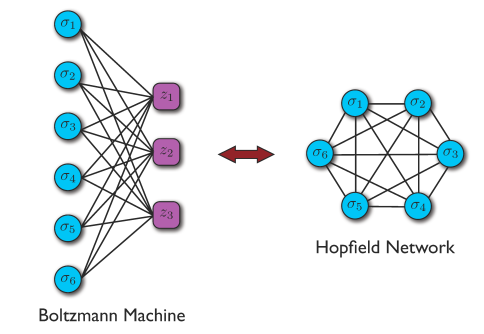
\includegraphics[width=0.7\textwidth]{img/duality_RBM_Hopfield.png}
    \caption{Correspondence between a two-layer restricted Boltzmann machine and an Hopfield neural network.}
    \label{fig:duality_RBM_Hopfield}
\end{figure}

\begin{observacion}
    La proporción entre la capa oculta ($P$) y la visible ($N$), definida matemáticamente como $\alpha = \lim_{N \to \infty} P/N$, equivale exactamente a la capacidad de almacenamiento de patrones en el modelo de Hopfield. Si la capa oculta es demasiado grande en relación con la visible (superando un umbral crítico), la red no aprende a generalizar, sino que cae en el overfitting (sobreajuste), al igual que una red de Hopfield colapsa si intentas ``forzarla'' a recordar demasiados patrones.
\end{observacion}